\documentclass[twoside]{IEEEtran}

\usepackage{amsmath}
\usepackage{tikz}

\bibliographystyle{IEEEtran}

\newcommand{\mult}{\nonscript\:}
\newcommand{\opoff}{{\operatorname{off}}}
\newcommand{\opout}{{\operatorname{out}}}
\newcommand{\opth}{{\operatorname{th}}}
\newcommand{\optotal}{{\operatorname{total}}}
\newcommand{\opx}{{\operatorname{x}}}

\begin{document}

\title{An Extension of the Construction of\\Power Conservative Equivalent Circuits for\\DC Networks containing Current Sources}
\author{Julian Ahrens}
\maketitle

\section{Introduction}
\label{section_introduction}

By the Th\'{e}venin Theorem, any electrical network between two terminals, containing only voltage sources, current sources, and resistors, can be replaced by an equivalent circuit consisting of a voltage source $V_{\opth}$ and a series resistance $R_{\opth}$.
However, the power dissipated by the series resistance is not necessarily the same as the combined power dissipated by the resistors of the original network.
In a recent paper~\cite{Bar20}, it was shown that, in the case where the original network does not contain any current sources, a \emph{power conservative} equivalent circuit can be constructed.
The term `power conservative' refers to the property of the equivalent circuit, that it exhibits the same amount of Joule heating as the original network under all conditions, i.e., the total power dissipated by the resistors of the equivalent circuit is the same as the total power dissipated by the resistors of the original network.
In the following, an extension of this construction to the case of networks containing both voltage and current sources is developed.
The construction is divided into two parts: in Section~\ref{section_power} an analysis of the power dissipated in the original network is performed and in Section~\ref{section_circuit} the equivalent circuit is introduced and the values of its elements determined.

\section{Power dissipation in a general network}
\label{section_power}

\begin{figure}
  \centering
  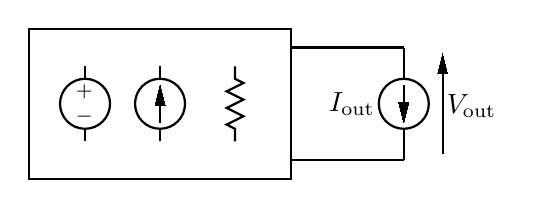
\begin{tikzpicture}[scale=2.54]
% dpic version 2020.06.01 option -g for TikZ and PGF 1.01
\ifx\dpiclw\undefined\newdimen\dpiclw\fi
\global\def\dpicdraw{\draw[line width=\dpiclw]}
\global\def\dpicstop{;}
\dpiclw=0.8bp
\dpiclw=0.8bp
\dpicdraw (0,0)
 --(0,0.0625)\dpicstop
\dpicdraw (0,0.1875) circle (0.049213in)\dpicstop
\draw (0,0.125) node{$_-$};
\draw (0,0.25) node{$_+$};
\dpicdraw (0,0.3125)
 --(0,0.375)\dpicstop
\dpicdraw (0.375,0)
 --(0.375,0.0625)\dpicstop
\dpicdraw (0.375,0.1875) circle (0.049213in)\dpicstop
\filldraw[line width=0bp](0.4,0.18125)
 --(0.375,0.28125)
 --(0.35,0.18125) --cycle\dpicstop
\dpicdraw (0.375,0.09375)
 --(0.375,0.258344)\dpicstop
\dpicdraw (0.375,0.3125)
 --(0.375,0.375)\dpicstop
\dpicdraw (0.75,0)
 --(0.75,0.0625)
 --(0.708333,0.083333)
 --(0.791667,0.125)
 --(0.708333,0.166667)
 --(0.791667,0.208333)
 --(0.708333,0.25)
 --(0.791667,0.291667)
 --(0.75,0.3125)
 --(0.75,0.375)\dpicstop
\dpicdraw (-0.28125,-0.1875) rectangle (1.03125,0.5625)\dpicstop
\dpicdraw (1.03125,0.46875)
 --(1.59375,0.46875)\dpicstop
\dpicdraw (1.59375,0.46875)
 --(1.59375,0.3125)\dpicstop
\dpicdraw (1.59375,0.1875) circle (0.049213in)\dpicstop
\filldraw[line width=0bp](1.56875,0.19375)
 --(1.59375,0.09375)
 --(1.61875,0.19375) --cycle\dpicstop
\dpicdraw (1.59375,0.28125)
 --(1.59375,0.116656)\dpicstop
\dpicdraw (1.59375,0.0625)
 --(1.59375,-0.09375)\dpicstop
\draw (1.46875,0.1875) node[left=-2bp]{$ I_{\opout}$};
\filldraw[line width=0bp](1.812935,0.3375)
 --(1.787935,0.4375)
 --(1.762935,0.3375) --cycle\dpicstop
\dpicdraw (1.787935,0.414594)
 --(1.787935,-0.0625)\dpicstop
\draw (1.787935,0.176047) node[right=-2bp]{$ V_{\opout}$};
\dpicdraw (1.59375,-0.09375)
 --(1.03125,-0.09375)\dpicstop
\end{tikzpicture}

  \caption{Electrical network with current load}
  \label{loaded_network}
\end{figure}

For the analysis of the power dissipated by the resistors in an electrical network consisting only of voltage sources, current sources, and resistors, a current load $I_{\opout}$ is attached to the two terminals of the network as shown in \figurename~\ref{loaded_network}.
In the following, the voltage across this load is denoted by $V_{\opout}$.
Furthermore, let $R_{k}$, $k = 0, \ldots, n - 1$, denote the values of the resistors in the network and let $V_{\opth}$ and $R_{\opth}$ denote the values of the voltage source and resistor of the Th\'{e}venin equivalent of the network, respectively.

Now examine a modified version of the network where all the sources are switched off, i.e., all voltage sources are replaced by a short circuit and all current sources are replaced by an open circuit.
The current through each of the resistors $R_{k}$ in this modified network is proportional to the current flowing through the terminals of the network, i.e., for each $k$, there exists a unique constant $c_{k}$ such that the current through the resistor $R_{k}$ is equal to $I_{k, \opoff} = I_{\opout} \mult c_{k}$.
In particular, the power dissipated by $R_{k}$ is equal to
\begin{equation}
    P_{k, \opoff}
  = I_{k, \opoff}^{2} \mult R_{k}
  = (I_{\opout} \mult c_{k})^{2} \mult R_{k}
  \enskip.
  \label{equation_power_k_off}
\end{equation}
Furthermore, since the modified network consists purely of resistors and its equivalent resistance is, by the Th\'{e}venin theorem, equal to $R_{\opth}$, the total power dissipated by the entire network is given by
\begin{equation}
    P_{\optotal, \opoff}
  = I_{\opout}^{2} \mult R_{\opth}
  \enskip.
  \label{equation_power_total_off}
\end{equation}
Now since the total power dissipated by the entire network has to be equal to the sum of all the power dissipated in each individual resistor, combining \eqref{equation_power_k_off}~and~\eqref{equation_power_total_off}, we obtain the equation
\begin{displaymath}
    I_{\opout}^{2} \mult R_{\opth}
  = \sum_{k} (I_{\opout} \mult c_{k})^{2} \mult R_{k}
  = I_{\opout}^{2} \mult \sum_{k} c_{k}^{2} \mult R_{k}
\end{displaymath}
and therefore
\begin{equation}
    \sum_{k} c_{k}^{2} \mult R_{k}
  = R_{\opth}
  \enskip.
  \label{equation_leading_coefficient}
\end{equation}

Returning to the original network, by the superposition principle, for each $k$, the current through the resistor $R_{k}$ is given by $I_{k} = I_{k, \opoff} + I_{k, 0} = I_{\opout} \mult c_{k} + I_{k, 0}$, where $I_{k, 0}$ denotes the current through the resistor at zero load current $I_{\opout}$.
Correspondingly, for each $k$, the power dissipated by the resistor $R_{k}$ is equal to
\begin{align*}
         P_{k}
     & = I_{k}^{2} \mult R_{k}
       = (I_{\opout} \mult c_{k} + I_{k, 0})^{2} \mult R_{k}
  \\ & = I_{\opout}^{2} \mult c_{k}^{2} \mult R_{k} + I_{\opout} \mult c_{k} \mult I_{k, 0} \cdot 2 \mult R_{k} + I_{k, 0}^{2} \mult R_{k}
  \enskip.
\end{align*}
Summing over all the resistors and applying~\eqref{equation_leading_coefficient} yields the total power dissipated by the network:
\begin{align}
         P_{\optotal}
     & = \sum_{k} P_{k}
  \nonumber \\ & = \sum_{k} \bigl( I_{\opout}^{2} \mult c_{k}^{2} \mult R_{k} + I_{\opout} \mult c_{k} \mult I_{k, 0} \cdot 2 \mult R_{k} + I_{k, 0}^{2} \mult R_{k} \bigr)
  \nonumber \\ & = I_{\opout}^{2} \mult \sum_{k} c_{k}^{2} \mult R_{k} + I_{\opout} \cdot 2 \mult \sum_{k} c_{k} \mult I_{k, 0} \mult R_{k} \nonumber \\ & \qquad + \sum_{k} I_{k, 0}^{2} \mult R_{k}
  \nonumber \\ & = I_{\opout}^{2} \mult R_{\opth} + I_{\opout} \cdot 2 \mult \sum_{k} c_{k} \mult I_{k, 0} \mult R_{k} + \sum_{k} I_{k, 0}^{2} \mult R_{k}
  \enskip.
  \label{equation_power_total}
\end{align}
In summary, the power dissipated in the network is a non-negative quadratic polynomial in $I_{\opout}$ with leading coefficient $R_{\opth}$.

\section{Power conservative equivalent circuit}
\label{section_circuit}

\begin{figure}
  \centering
  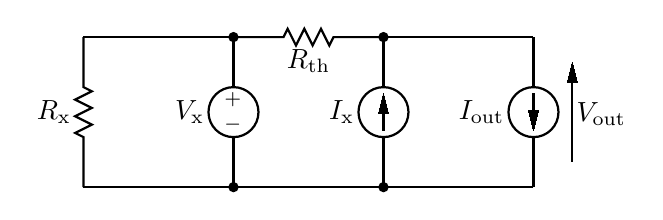
\begin{tikzpicture}[scale=2.54]
% dpic version 2020.06.01 option -g for TikZ and PGF 1.01
\ifx\dpiclw\undefined\newdimen\dpiclw\fi
\global\def\dpicdraw{\draw[line width=\dpiclw]}
\global\def\dpicstop{;}
\dpiclw=0.8bp
\dpiclw=0.8bp
\dpicdraw (0,0)
 --(-0,0.25)
 --(-0.041667,0.270833)
 --(0.041667,0.3125)
 --(-0.041667,0.354167)
 --(0.041667,0.395833)
 --(-0.041667,0.4375)
 --(0.041667,0.479167)
 --(0,0.5)
 --(0,0.75)\dpicstop
\draw (-0.041667,0.375) node[left=-2bp]{$ R_{\opx}$};
\dpicdraw (0,0.75)
 --(0.75,0.75)\dpicstop
\dpicdraw (0.75,0.75)
 --(1,0.75)
 --(1.020833,0.791667)
 --(1.0625,0.708333)
 --(1.104167,0.791667)
 --(1.145833,0.708333)
 --(1.1875,0.791667)
 --(1.229167,0.708333)
 --(1.25,0.75)
 --(1.5,0.75)\dpicstop
\draw (1.125,0.708333) node[below=-2bp]{$ R_{\opth}$};
\dpicdraw (1.5,0.75)
 --(2.25,0.75)\dpicstop
\dpicdraw (2.25,0.75)
 --(2.25,0.5)\dpicstop
\dpicdraw (2.25,0.375) circle (0.049213in)\dpicstop
\filldraw[line width=0bp](2.225,0.38125)
 --(2.25,0.28125)
 --(2.275,0.38125) --cycle\dpicstop
\dpicdraw (2.25,0.46875)
 --(2.25,0.304156)\dpicstop
\dpicdraw (2.25,0.25)
 --(2.25,0)\dpicstop
\draw (2.125,0.375) node[left=-2bp]{$ I_{\opout}$};
\filldraw[line width=0bp](2.469185,0.525)
 --(2.444185,0.625)
 --(2.419185,0.525) --cycle\dpicstop
\dpicdraw (2.444185,0.602094)
 --(2.444185,0.125)\dpicstop
\draw (2.444185,0.363547) node[right=-2bp]{$ V_{\opout}$};
\dpicdraw (2.25,0)
 --(1.5,0)\dpicstop
\dpicdraw[fill=black](1.5,0) circle (0.007874in)\dpicstop
\dpicdraw (1.5,0)
 --(1.5,0.25)\dpicstop
\dpicdraw (1.5,0.375) circle (0.049213in)\dpicstop
\filldraw[line width=0bp](1.525,0.36875)
 --(1.5,0.46875)
 --(1.475,0.36875) --cycle\dpicstop
\dpicdraw (1.5,0.28125)
 --(1.5,0.445844)\dpicstop
\dpicdraw (1.5,0.5)
 --(1.5,0.75)\dpicstop
\draw (1.375,0.375) node[left=-2bp]{$ I_{\opx}$};
\dpicdraw[fill=black](1.5,0.75) circle (0.007874in)\dpicstop
\dpicdraw (1.5,0)
 --(0.75,0)\dpicstop
\dpicdraw[fill=black](0.75,0) circle (0.007874in)\dpicstop
\dpicdraw (0.75,0)
 --(0.75,0.25)\dpicstop
\dpicdraw (0.75,0.375) circle (0.049213in)\dpicstop
\draw (0.75,0.3125) node{$_-$};
\draw (0.75,0.4375) node{$_+$};
\dpicdraw (0.75,0.5)
 --(0.75,0.75)\dpicstop
\draw (0.625,0.375) node[left=-2bp]{$ V_{\opx}$};
\dpicdraw[fill=black](0.75,0.75) circle (0.007874in)\dpicstop
\dpicdraw (0.75,0)
 --(0,0)\dpicstop
\end{tikzpicture}

  \caption{Power conservative equivalent circuit with current load}
  \label{equivalent_circuit}
\end{figure}

In order to obtain a power conservative equivalent circuit, a circuit exhibiting both the same electrical properites as the original network and the same power dissipation in its resistors has to be found.
The Th\'{e}venin theorem reduces the problem of electrical equivalence to the problem of finding a network satisfying $V_{\opout} = V_{\opth} - I_{\opout} \mult R_{\opth}$.

As shown in Section~\ref{section_power}, the power dissipated by the resistors in the network is a non-negative quadratic polynomial in $I_{\opout}$ with leading coefficient $R_{\opth}$.
Elementary algebra shows that such a polynomial can always be parametrized as
\begin{equation}
    P_{\optotal}
  = (I_{\opout} - I_{\opx})^{2} \mult R_{\opth} + P_{\opx}
  \label{equation_parametrization}
\end{equation}
The parameters $P_{\opx} \ge 0$ and $I_{\opx}$ are equal to the minimum power dissipated by the resistors in the network and the current at which this minimum is attained, respectively.

One possibility of obtaining a power conservative equivalent circuit is shown in \figurename~\ref{equivalent_circuit}.
In order to achieve equivalence, the values of the elements $R_{\opth}$ and $I_{\opx}$ have to be chosen as the values appearing in~\eqref{equation_parametrization} and the values of the elements $R_{\opx}$ and $V_{\opx}$ have to be chosen according to the following equations:
\begin{displaymath}
    V_{\opx}
  = V_{\opth} - I_{\opx} \mult R_{\opth}
  \qquad
    R_{\opx}
  = \frac{V_{\opx}^{2}}{P_{\opx}}
\end{displaymath}
In the case $P_{\opx} = 0$, the resistor $R_{\opx}$ can be omitted.

It is a straighforward exercise to verify that, as long as $V_{\opx} \ne 0$ or $P_{\opx} = 0$, the obtained circuit is indeed both power conservative and electrically equivalent.
The construction fails in the case where $V_{\opx} = 0$ and $P_{\opx} \ne 0$ since then the resistor $R_{\opx}$ is unable to dissipate power.
However, as long as $I_{\opx} \ne 0$, a resistor of value $P_{\opx} / I_{\opx}^{2}$ may be connected in series with $I_{\opx}$ instead.
If both $V_{\opx} = 0$ and $I_{\opx} = 0$ and yet still $P_{\opx} \ne 0$, a separate source has to be added to the circuit and a suitable resistor connected across its terminals.
Since in each of these special cases some of the elements disappear from the circuit, a power conservative equivalent circuit can nevertheless always be constructed from at most four elements.
These four elements clearly correspond to the four degrees of freedom $V_{\opth}$, $R_{\opth}$, $P_{\opx}$, and $I_{\opx}$ in the above characterization of the network.

\bibliography{main}

\end{document}

